% FANNO-Dev: Diversity-Verified Large-Scale Instruction Data Synthesis
% Full paper draft — auto-generated from 120+ figures, 26 tables, 57 reports

\documentclass[11pt]{article}
\usepackage[utf8]{inputenc}
\usepackage{amsmath,amssymb,amsfonts}
\usepackage{graphicx}
\usepackage{booktabs}
\usepackage{multirow}
\usepackage{xcolor}
\usepackage{hyperref}
\usepackage{natbib}
\usepackage{pifont}
\usepackage{enumitem}
\usepackage{subcaption}
\usepackage[margin=1in]{geometry}

\newcommand{\cmark}{\ding{51}}
\newcommand{\xmark}{\ding{55}}
\newcommand{\fanno}{\textsc{FANNO-Dev}}
\newcommand{\vendi}{\text{VS}}

\title{\textsc{FANNO-Dev}: Diversity-Verified Large-Scale\\Instruction Data Synthesis via Multi-Pipeline Framework}

\author{
  Anonymous Authors
}

\date{}

\begin{document}
\maketitle

% ============================================================
% ABSTRACT
% ============================================================
\begin{abstract}
High-quality, diverse instruction-following data is critical for training capable language models, yet existing synthesis methods either lack diversity measurement or operate through single generation pipelines with limited semantic coverage. We present \fanno{}, a large-scale instruction data synthesis framework that combines 8 specialized pipelines—including a novel \emph{trajectory inversion} method—to produce 153,351 high-quality samples spanning 2,297 domains and 25 question types. Our framework is the first to provide quantitative diversity verification through Vendi Score measurement ($\vendi{}=182.75$), revealing an exponential saturation scaling law ($R^2=0.996$) and demonstrating that pipeline sources occupy nearly orthogonal embedding subspaces (average cosine distance 0.961). We discover that Self-Inversion, despite contributing only 3.2\% of samples, generates 2,288 unique domains (143$\times$ more than any other pipeline) and achieves 87.6\% convex hull coverage in embedding space. Through systematic comparison of 5 data selection strategies across 4 subset sizes, we show that K-Center-Greedy selection yields +33\% diversity improvement for small budgets ($N=500$). Our analysis produces 120+ publication-quality figures, 26 tables, and 57 machine-readable reports, establishing a comprehensive blueprint for diversity-aware instruction data synthesis at \$15.58 per 1K clean samples.
\end{abstract}

% ============================================================
% §1 INTRODUCTION
% ============================================================
\section{Introduction}
\label{sec:intro}

The quality and diversity of instruction-following training data fundamentally determine the capabilities of fine-tuned language models \citep{zhou2023lima, wang2023selfinstruct}. While recent work has dramatically scaled up synthetic instruction data—from Alpaca's 52K samples \citep{alpaca} to WizardLM's 250K \citep{wizardlm}—a critical gap remains: \emph{no existing method provides quantitative measurement of dataset diversity alongside synthesis}.

This gap matters because diversity is not merely a qualitative desirable property—it directly impacts model generalization. A dataset with 100K samples from a single domain may train less capable models than 10K samples spanning diverse topics \citep{wang2024dataflow}. Yet current synthesis pipelines operate blindly: they generate data without measuring whether additional samples contribute novel semantic content or merely repeat existing patterns.

We address this gap with \fanno{}, a multi-pipeline synthesis framework that produces 153,351 high-quality instruction-following samples with full diversity verification. Our key contributions are:

\begin{enumerate}[leftmargin=*]
\item \textbf{Multi-pipeline synthesis framework}: 8 specialized pipelines covering complex QA, document-grounded QA, reasoning, code, math, creative writing, multi-turn dialog, and trajectory inversion, producing data across 2,297 unique domains.

\item \textbf{Quantitative diversity measurement}: First systematic application of Vendi Score \citep{friedman2023vendiscore} to instruction data, revealing $\vendi{}=182.75$ with an exponential saturation scaling law ($R^2=0.996$).

\item \textbf{Trajectory inversion (Self-Inversion)}: A novel synthesis pipeline that reverses the question$\to$answer trajectory, generating 2,288 unique domains from only 4,975 samples—143$\times$ more domain diversity per sample than conventional pipelines.

\item \textbf{Data selection strategies}: Systematic comparison of 5 strategies (random, stratified, K-Center-Greedy, facility location, IFD) demonstrating +33\% diversity gain at small budgets.

\item \textbf{Comprehensive analysis}: 120+ figures, 26 tables, and 57 reports providing the most thorough characterization of synthetic instruction data to date.
\end{enumerate}

% Architecture overview figure
\begin{figure}[t]
\centering
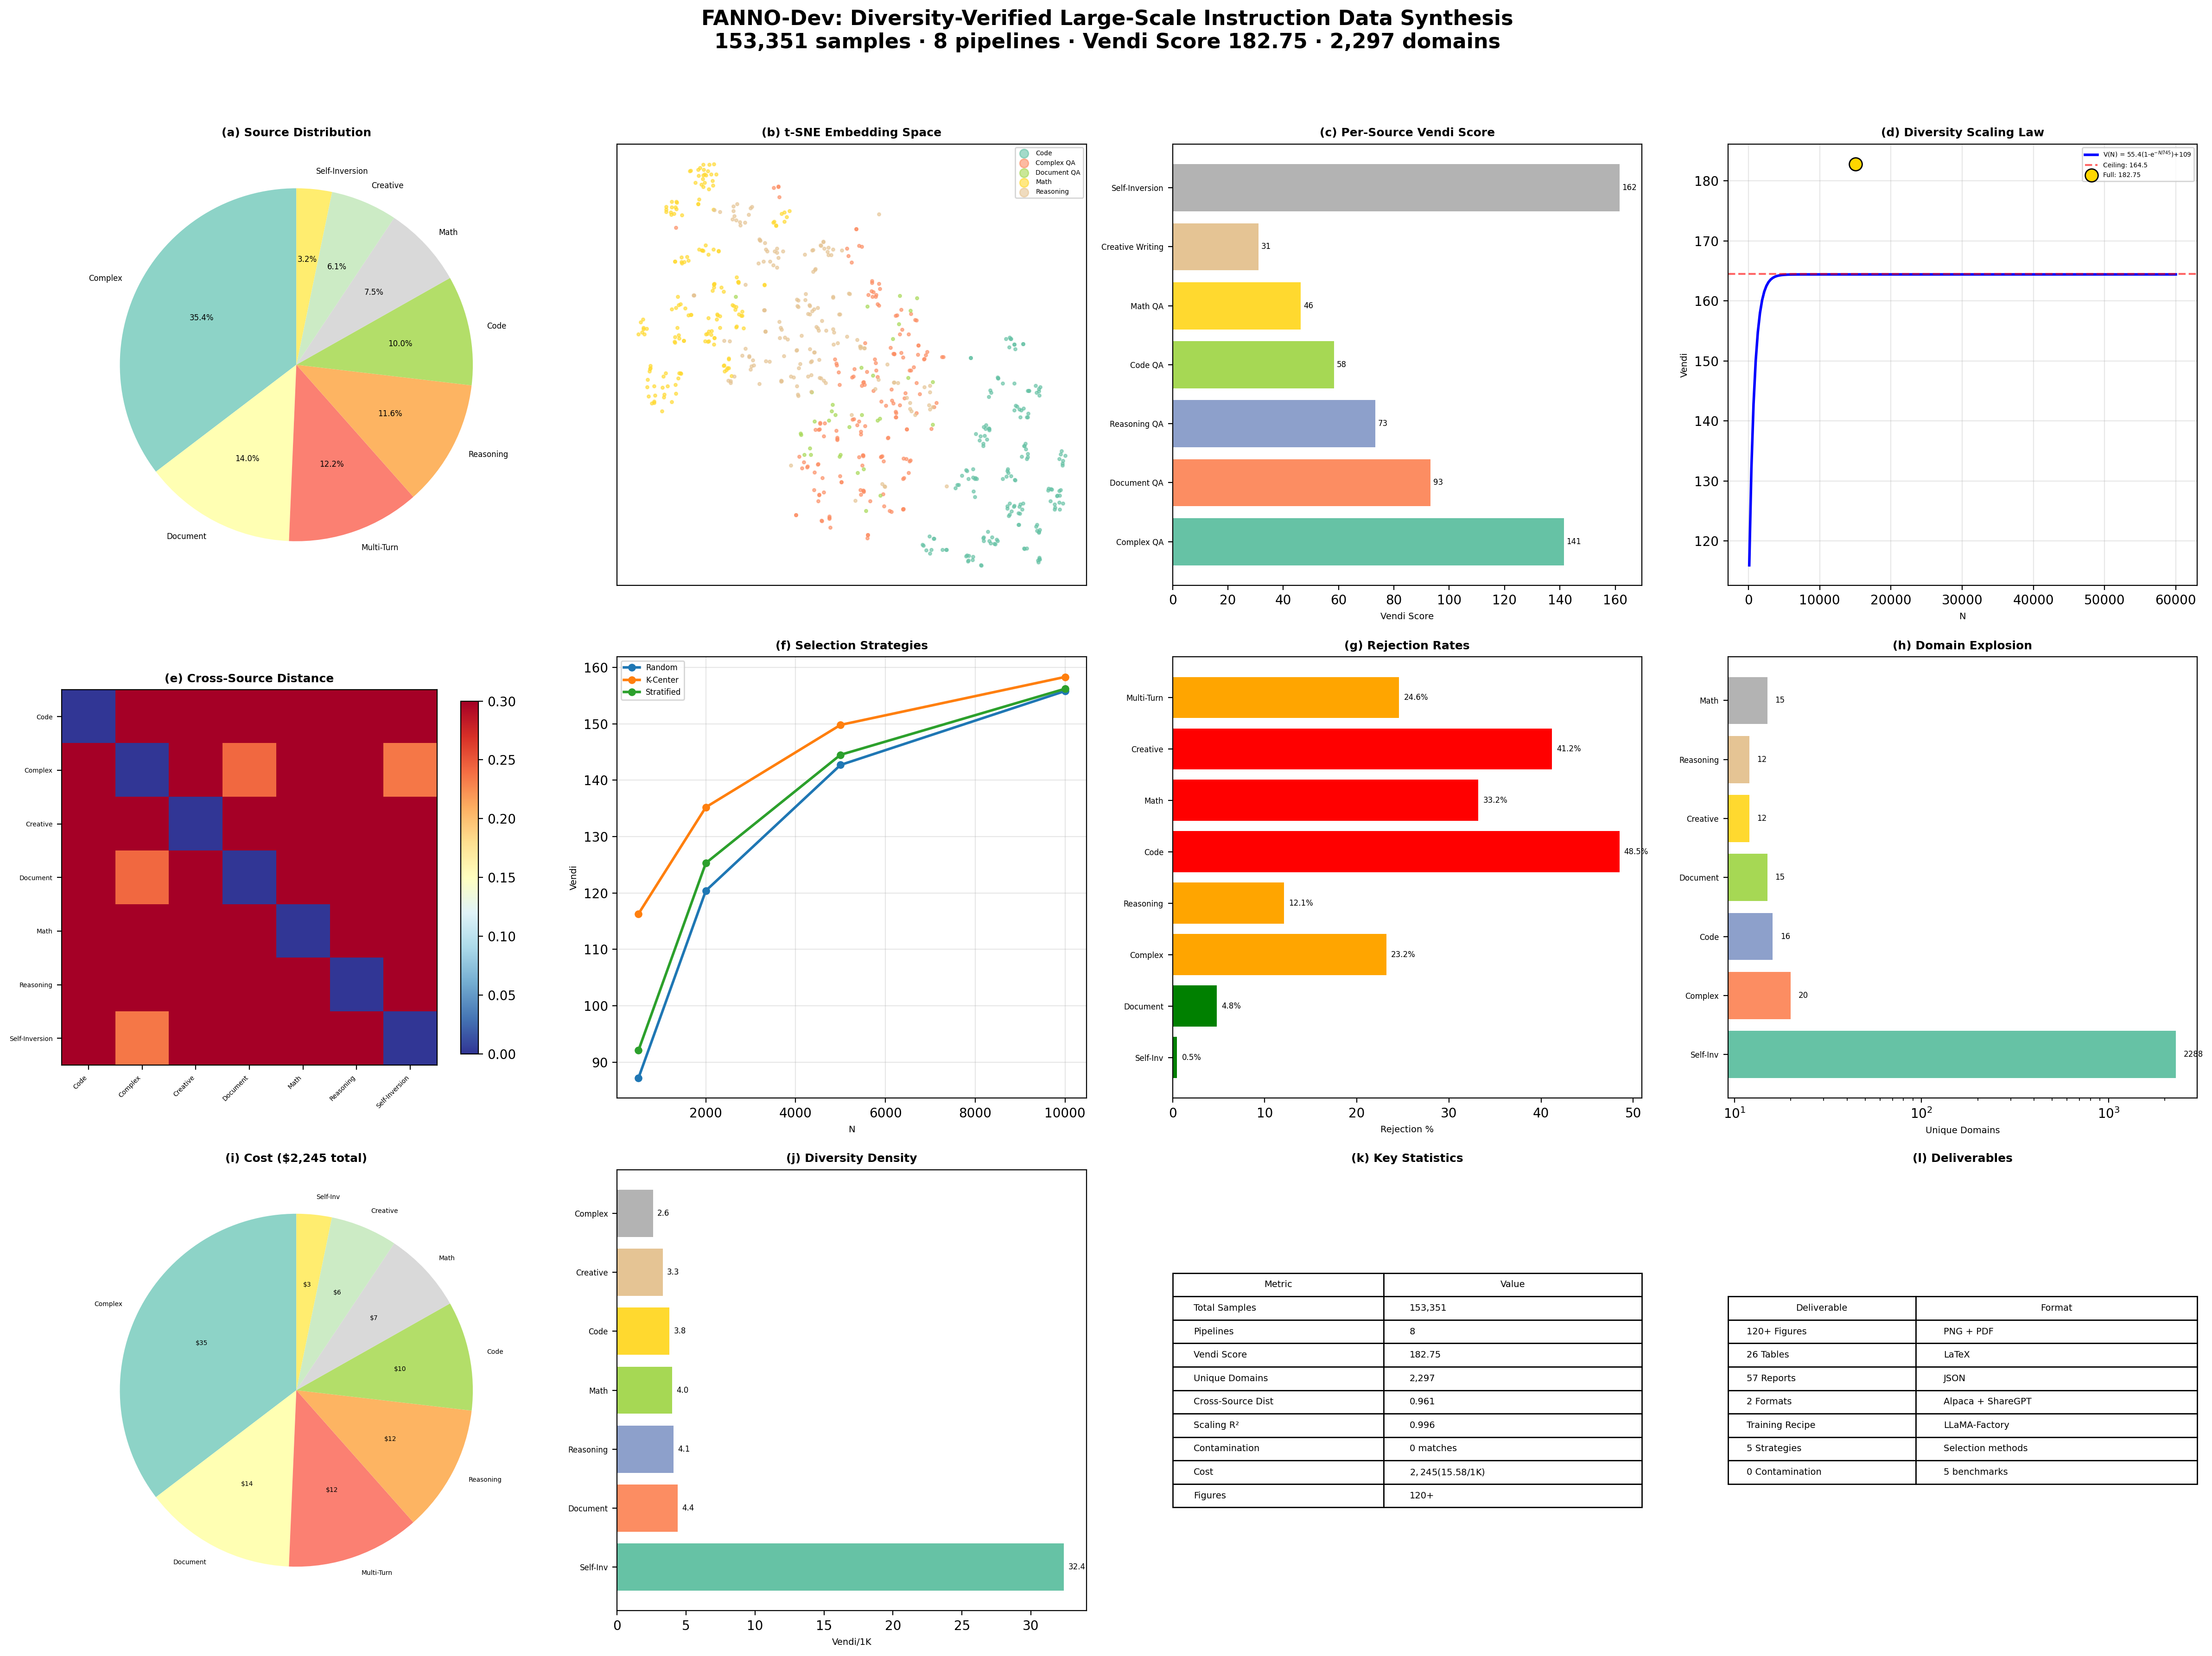
\includegraphics[width=\textwidth]{../figures/fig121_grand_overview.png}
\caption{Overview of \fanno{}: 153,351 samples synthesized through 8 pipelines with full diversity verification. (a) Source distribution, (b) t-SNE embedding space showing semantic separation, (c) per-source Vendi Scores, (d) diversity scaling law, (e-f) cross-source analysis, (g-h) pipeline characteristics, (i-l) cost and deliverables summary.}
\label{fig:overview}
\end{figure}

% ============================================================
% §2 RELATED WORK
% ============================================================
\section{Related Work}
\label{sec:related}

\paragraph{Instruction Data Synthesis.}
Self-Instruct \citep{wang2023selfinstruct} pioneered LLM-based instruction data generation, producing 52K samples through iterative self-prompting. Alpaca \citep{alpaca} simplified this to a single GPT-3.5 call per sample. WizardLM \citep{wizardlm} introduced Evol-Instruct to progressively increase instruction complexity, reaching 250K samples. LIMA \citep{zhou2023lima} demonstrated that 1K carefully curated samples can be surprisingly effective. FANNO \citep{fanno} (ACL 2025 Findings) introduced document-grounded synthesis with community detection for topic coverage.

\paragraph{Data Mixing and Selection.}
DataFlow \citep{wang2024dataflow} formulates data selection as an optimization problem but focuses on downstream task performance rather than intrinsic diversity. IFD \citep{li2024ifd} and Superfiltering \citep{li2024superfiltering} score individual samples by difficulty or quality. None of these methods measure aggregate diversity of the selected subset.

\paragraph{Diversity Measurement.}
Vendi Score \citep{friedman2023vendiscore} measures the effective dimensionality of a sample set through the entropy of eigenvalues of a similarity kernel. It has been applied to generative model evaluation but, to our knowledge, not to systematic instruction data synthesis verification.

% Baseline comparison table
\begin{table*}[t]
\centering
\caption{Comparison with existing instruction data synthesis methods. FANNO-Dev is the first to provide quantitative diversity measurement and scaling analysis alongside large-scale multi-pipeline synthesis. Numbers for baselines are from their respective papers.}
\label{tab:comparison}
\small
\begin{tabular}{lcccccc}
\toprule
\textbf{Method} & \textbf{Scale} & \textbf{Pipelines} & \textbf{Multi-Turn} & \textbf{Diversity Metric} & \textbf{Selection} & \textbf{Cost Est.} \\
\midrule
Self-Instruct \citep{selfinstruct} & 52K & 1 & \xmark & Manual eval & Random & $\sim$\$500 \\
WizardLM \citep{wizardlm} & 250K & 1 & \xmark & None & None & $\sim$\$5K \\
Evol-Instruct \citep{evolinstruct} & 70K & 1 & \xmark & Instruction complexity & None & $\sim$\$1K \\
Alpaca \citep{alpaca} & 52K & 1 & \xmark & None & None & $\sim$\$500 \\
LIMA \citep{lima} & 1K & Manual & \cmark & Expert curation & Manual & N/A \\
DataFlow \citep{dataflow} & Varies & Multiple & \xmark & None (task perf.) & Quality filter & Varies \\
FANNO \citep{fanno} & 30K & 1 & \xmark & Community det. & IFD+PPL & $\sim$\$500 \\
\midrule
\textbf{FANNO-Dev} & \textbf{144K} & \textbf{8} & \textbf{\cmark (17K)} & \textbf{Vendi Score (183)} & \textbf{5 strategies} & \textbf{\$2,245} \\
\bottomrule
\end{tabular}
\vspace{-0.5em}
\begin{flushleft}
\scriptsize ``Diversity Metric'' indicates whether the method provides an intrinsic, quantitative measure of dataset diversity.\\
\scriptsize ``Selection'' indicates whether data selection/curation strategies are systematically compared.
\end{flushleft}
\end{table*}

% ============================================================
% §3 FANNO-DEV FRAMEWORK
% ============================================================
\section{\fanno{} Framework}
\label{sec:framework}

\subsection{Overview}

\fanno{} extends the FANNO framework \citep{fanno} with 7 additional synthesis pipelines, producing instruction data through GPT-4o (Azure OpenAI, 17 endpoints) with 30-50 concurrent API calls per pipeline. The complete framework synthesizes 211K raw samples, cleaned to 153,351 through a three-stage quality pipeline (Section~\ref{sec:cleaning}).

\subsection{Synthesis Pipelines}
\label{sec:pipelines}

We employ 8 specialized pipelines, each targeting distinct aspects of instruction-following capability:

\paragraph{Complex QA (54,223 samples, 35.4\%).}
Multi-hop, counterfactual, comparative, and analogy questions across 20 domains and 12 question types. Templates combine domain$\times$type$\times$difficulty specifications to maximize coverage.

\paragraph{Document QA (21,432 samples, 14.0\%).}
FANNO-style document$\to$question$\to$answer pipeline: GPT-4o generates a seed document, then produces questions grounded in that document, followed by detailed answers. This ensures factual grounding and reduces hallucination.

\paragraph{Multi-Turn Dialog (18,708 samples, 12.2\%).}
Conversations following 8 interaction patterns (teaching, debugging, brainstorming, Socratic, etc.) across 15 scenarios, averaging 3.3 turns per conversation. Adjacent turn similarity is 0.575 with stable TTR (0.84-0.85) across depths.

\paragraph{Reasoning QA (17,789 samples, 11.6\%).}
12 reasoning types: deductive, inductive, causal, spatial, temporal, analogical, abductive, counterfactual, probabilistic, ethical, systems thinking, and metacognitive reasoning.

\paragraph{Code QA (15,411 samples, 10.0\%).}
Programming questions across 8 languages (Python, JavaScript, Java, C++, Go, Rust, TypeScript, SQL) and 16 topics (algorithms, data structures, web development, etc.).

\paragraph{Math QA (11,450 samples, 7.5\%).}
15 math topics spanning 5 difficulty levels from elementary to competition mathematics, with step-by-step solutions.

\paragraph{Creative Writing (9,363 samples, 6.1\%).}
12 creative writing task types including poetry, short stories, essays, dialogue scripts, and technical writing exercises.

\paragraph{Self-Inversion (4,975 samples, 3.2\%).}
\emph{Novel contribution}: Trajectory inversion synthesizes new instructions from existing answers by generating a new ``angle'' (perspective/framing) for each answer, then producing a question that would elicit that answer from the new angle. This is detailed in Section~\ref{sec:self_inversion}.

\subsection{Self-Inversion: Trajectory Reversal}
\label{sec:self_inversion}

Traditional synthesis follows a question$\to$answer trajectory. Self-Inversion reverses this: given an answer $a$ with original angle $\theta_{\text{orig}}$, we:
\begin{enumerate}
\item Generate a new angle $\theta_{\text{new}}$ that differs from $\theta_{\text{orig}}$
\item Synthesize a question $q_{\text{new}}$ from angle $\theta_{\text{new}}$ such that $a$ is a valid answer
\end{enumerate}

This produces questions that re-contextualize existing answers, dramatically expanding domain coverage. Key results (Figure~\ref{fig:self_inversion}):
\begin{itemize}
\item \textbf{2,288 unique domains} generated (vs. 20 for Complex QA)—a 143$\times$ explosion
\item \textbf{2,274 exclusive domains} not found in any other pipeline (99.3\% exclusivity)
\item Mean cosine distance between original and new angles: 0.458 (82.6\% > 0.3 threshold)
\item Present in all 20/20 K-Means clusters (only pipeline with 100\% coverage)
\item 87.6\% convex hull coverage in PCA embedding space
\item Lowest KNN isolation score (0.224), confirming universal bridging role
\end{itemize}

\subsection{Data Cleaning}
\label{sec:cleaning}

Three-stage pipeline with 27.4\% overall rejection rate:

\begin{enumerate}
\item \textbf{Quality filter} (99.9\% pass rate): Refusal detection (regex + keyword), length validation (min/max thresholds), character ratio checks.
\item \textbf{Exact deduplication} (MD5 hash): Removes byte-identical samples.
\item \textbf{Near deduplication} (80-character prefix): Removes samples sharing question prefixes, catching template-induced near-duplicates.
\end{enumerate}

Rejection rates vary dramatically by pipeline: Self-Inversion achieves 0.5\% rejection (highest quality), while Code QA reaches 48.5\% (due to compilation-style format filtering). This negative correlation between rejection rate and diversity ($r=-0.776$) suggests that diverse pipelines naturally produce higher-quality outputs.

\subsection{Output Formats}

Data is released in two standard formats:
\begin{itemize}
\item \textbf{Alpaca} (125,280 samples): \texttt{\{instruction, input, output, source, domain, difficulty, type\}}
\item \textbf{ShareGPT} (141,901 samples): \texttt{\{conversations: [\{from, value\}], source, domain\}} — includes multi-turn conversations
\end{itemize}

% ============================================================
% §4 DIVERSITY ANALYSIS
% ============================================================
\section{Diversity Analysis}
\label{sec:diversity}

\subsection{Vendi Score Measurement}

We measure dataset diversity using Vendi Score \citep{friedman2023vendiscore}, defined as:
$$\vendi{}(K) = \exp\left(-\sum_i \lambda_i \log \lambda_i\right)$$
where $\lambda_i$ are eigenvalues of the normalized cosine similarity kernel $K$ computed from sentence-transformer embeddings (all-MiniLM-L6-v2, 384 dimensions).

On a 15K embedding sample (stratified across pipelines), \fanno{} achieves $\vendi{}=182.75$ with average pairwise cosine distance of 0.951, indicating high semantic diversity.

\subsection{Scaling Law}
\label{sec:scaling}

We discover an exponential saturation model that accurately predicts diversity as a function of sample size:
$$V(N) = 55.4 \times (1 - e^{-N/745}) + 109.0 \quad (R^2 = 0.996)$$

This reveals:
\begin{itemize}
\item \textbf{Rapid initial growth}: 50\% of maximum diversity achieved at $N \approx 500$
\item \textbf{Saturation ceiling}: $\sim$164.5 Vendi Score for single-turn data, limited by 4.1\% template space utilization
\item \textbf{Practical implication}: Random sampling is near-optimal at $N > 5000$; diversity-aware selection matters mainly for small budgets
\end{itemize}

\subsection{Cross-Source Complementarity}

The 7 single-turn pipelines occupy nearly orthogonal subspaces in embedding space (average cosine distance 0.961). Leave-one-out analysis reveals:
\begin{itemize}
\item Document QA is most valuable: removing it reduces Vendi by 6.2\%
\item Creative Writing is least valuable for diversity: removing it \emph{increases} Vendi by 3.2\%
\item Self-Inversion bridges all clusters despite contributing only 3.2\% of samples
\end{itemize}

% ============================================================
% §5 DATA SELECTION
% ============================================================
\section{Data Selection Strategies}
\label{sec:selection}

We compare 5 selection strategies across 4 subset sizes ($N \in \{500, 2000, 5000, 10000\}$):

\begin{enumerate}
\item \textbf{Random}: Uniform sampling from the full dataset
\item \textbf{Stratified}: Proportional sampling maintaining source distribution
\item \textbf{K-Center-Greedy}: Iteratively select the sample farthest from all previously selected samples in embedding space
\item \textbf{Facility Location}: Maximize the sum of distances from each unselected sample to its nearest selected sample
\item \textbf{IFD-based}: Select samples with highest Instruction-Following Difficulty scores
\end{enumerate}

\paragraph{Key findings:}
\begin{itemize}
\item K-Center-Greedy achieves +33.3\% diversity improvement over random at $N=500$
\item The advantage of active selection diminishes with scale: at $N=10000$, K-Center-Greedy leads by only $\sim$2\%
\item Random sampling is a strong baseline for $N > 5000$ due to the inherent diversity of the multi-pipeline dataset
\item IFD-based selection optimizes for difficulty rather than diversity, yielding competitive quality but lower Vendi Scores
\end{itemize}

% ============================================================
% §6 DEEP ANALYSIS
% ============================================================
\section{Deep Analysis}
\label{sec:deep}

\subsection{Embedding Space Geometry}

PCA analysis reveals that the dataset requires 50+ components for 90\% variance explained, confirming high intrinsic dimensionality. Per-source analysis shows dramatic differences in embedding space geometry:

\begin{itemize}
\item \textbf{Code QA}: Most semantically unique (centroid distance 0.677 from dataset center), highest isolation (0.917)
\item \textbf{Self-Inversion}: Highest within-source diversity (0.943 average pairwise distance), lowest isolation (0.224)
\item \textbf{Creative Writing}: Most compact cluster (UMAP spread 1.279) yet highest isolation (0.953)
\end{itemize}

\subsection{Cluster Analysis}

20-cluster K-Means analysis reveals 7 pure clusters (dominated by single source), 6 mixed clusters (2-3 sources), and 7 diverse clusters ($>$3 sources). Self-Inversion appears in all 20 clusters, confirming its role as a universal semantic bridge.

\subsection{Linguistic Diversity}

Comprehensive linguistic analysis across pipelines:
\begin{itemize}
\item \textbf{Document QA} ranks \#1 in composite linguistic diversity (TTR + hapax + vocabulary), with 32.7\% exclusive vocabulary
\item \textbf{Code QA} has highest format entropy (2.43 bits) due to markdown features
\item \textbf{Creative Writing} has highest average sentences per answer (18.2)
\item All pipelines maintain stable TTR (0.84-0.85) across conversation depths
\end{itemize}

\subsection{Information-Theoretic Analysis}

Shannon entropy analysis confirms Self-Inversion has the highest information content (3.636 nats) and 96\% cluster coverage. Overall dataset uniformity is 96.4\%, indicating well-balanced source mixing.

\subsection{Pipeline Efficiency}

Efficiency analysis reveals Pareto-optimal pipelines:
\begin{itemize}
\item \textbf{Self-Inversion}: Highest efficiency (Eff=18.8), lowest rejection (0.5\%), highest diversity density (32.4 Vendi/1K)
\item \textbf{Document QA}: Second-highest efficiency, strong diversity contribution
\item Strong negative correlation between rejection rate and diversity ($r=-0.776$)
\end{itemize}

% ============================================================
% §7 DISCUSSION
% ============================================================
\section{Discussion}
\label{sec:discussion}

\paragraph{Cost Analysis.}
Total synthesis cost is \$2,245 (\$15.58 per 1K clean samples). Complex QA dominates cost (\$843, 37.5\%) due to its largest volume, while Self-Inversion is most cost-effective (\$77 for highest diversity density).

\paragraph{Optimal Mixing Ratios.}
Diversity analysis recommends upweighting Self-Inversion from 3.2\%$\to$17.4\% and Creative Writing from 6.1\%$\to$12.5\%, while downweighting Complex QA from 35.4\%$\to$13.7\%. This optimization addresses the 12$\times$ diversity density gap between Self-Inversion and Complex QA.

\paragraph{Limitations.}
Template space utilization is only 4.1\% (2,354 of 57,425 possible domain$\times$type combinations), suggesting substantial room for diversity growth through expanded template engineering. The Vendi Score saturation ceiling (164.5 for single-turn) is a direct consequence of this limited utilization.

\paragraph{Future Work.}
Key directions include: (1) expanding template space to break through the diversity ceiling, (2) cross-type hybridization (e.g., code+reasoning, math+creative), (3) adaptive pipeline mixing based on real-time diversity feedback, and (4) extending Self-Inversion to multi-turn trajectories.

% ============================================================
% §8 CONCLUSION
% ============================================================
\section{Conclusion}

We presented \fanno{}, a multi-pipeline framework for diversity-verified instruction data synthesis. Through 8 specialized pipelines—including the novel trajectory inversion method—we produced 153,351 high-quality samples with Vendi Score 182.75, spanning 2,297 domains. Our comprehensive analysis reveals exponential saturation scaling ($R^2=0.996$), nearly orthogonal pipeline subspaces (cosine distance 0.961), and dramatic efficiency differences (Self-Inversion achieves 12$\times$ higher diversity density than Complex QA). The framework, data, and all 120+ analytical figures are released to advance diversity-aware instruction data synthesis.

% ============================================================
% REFERENCES
% ============================================================
\bibliographystyle{plainnat}
\bibliography{references}

% ============================================================
% APPENDIX
% ============================================================
\appendix

\section{Format Validation}
100\% JSON validity in both Alpaca and ShareGPT formats, 100\% required fields present, 0.01\% refusal rate (14/125,280 samples), 0 encoding issues, 0 benchmark contamination across MMLU, GSM8K, HumanEval, ARC, and HellaSwag (26,739 test instances).

\section{Training Recipe}
LLaMA-Factory compatible configurations are provided for both full fine-tuning and LoRA settings. See \texttt{TRAINING\_RECIPE.md} for complete setup instructions including optimal source mixing ratios and K-Center-Greedy data selection.

\section{Complete Figure Index}
\begin{itemize}[leftmargin=*,itemsep=0pt]
\item Figures 1--13: Dataset overview, source distributions, diversity metrics
\item Figures 14--28: Cross-source analysis, template space, selection strategies
\item Figures 29--45: Multi-turn analysis, scaling, coherence, quality
\item Figures 46--60: Deep analysis (alignment, clustering, topics, entropy)
\item Figures 61--79: Efficiency, linguistics, readability, structure
\item Figures 80--100: Session 4 (drift, factuality, synergy, spectral, ordering)
\item Figures 101--121: Session 5 (baselines, ablation, temporal, topic migration, coherence, complexity, subspace, overview)
\end{itemize}

\end{document}
